\documentclass[sigplan]{acmart}

\usepackage{booktabs} % For formal tables

\newcommand{\shellcmd}[1]{\\\texttt{\$ #1}}

% Copyright
%\setcopyright{none}
%\setcopyright{acmcopyright}
%\setcopyright{acmlicensed}
\setcopyright{rightsretained}
%\setcopyright{usgov}
%\setcopyright{usgovmixed}
%\setcopyright{cagov}
%\setcopyright{cagovmixed}


\newenvironment{packed_itemize}{
\begin{itemize}
  \setlength{\itemsep}{1pt}
  \setlength{\parskip}{0pt}
  \setlength{\parsep}{0pt}
}{\end{itemize}}

% DOI
\acmDOI{10.1145/3229762.3229764}

% ISBN
\acmISBN{978-1-4503-5923-8}

%Conference
\acmConference[ReQuEST at ASPLOS'18]{1st ACM Reproducible Quality-Efficient Systems Tournament on Co-designing Pareto-efficient Deep Learning}{March 2018}{Williamsburg, VA, USA}
\acmYear{2018}
\copyrightyear{2018}

%\acmPrice{15.00}

%\acmBadgeL[http://ctuning.org/ae/ppopp2016.html]{ae-logo}
%\acmBadgeR[http://ctuning.org/ae/ppopp2016.html]{ae-logo}


\begin{document}

\title{Optimizing Deep Learning Workloads on ARM GPU with TVM}
% \titlenote{Produces the permission block, and copyright information}
%\subtitle{Extended Abstract}
%\subtitlenote{The full version of the author's guide is available as \texttt{acmart.pdf} document}

\author{Lianmin Zheng}
\affiliation{\institution{Shanghai Jiao Tong University}}
\email{mercy_zheng@sjtu.edu.cn}

\author{Tianqi Chen}
\affiliation{\institution{University of Washington}}
\email{tqchen@cs.washington.edu}

\renewcommand{\shortauthors}{}
\renewcommand{\shorttitle}{}

% The default list of authors is too long for headers.
%\renewcommand{\shortauthors}{B. Trovato et al.}


\begin{abstract}
With the great success of deep learning, the demand for deploying deep neural networks to mobile devices is 
growing rapidly. However, current popular deep learning frameworks are often poorly optimized for mobile devices,
especially mobile GPU.
In this paper, we follow the pipeline proposed by TVM/NNVM, and optimize both kernel implementations and dataflow graph for ARM Mali GPU.
Compared with vendor-provided ARM Compute Library,  our kernel implementations and end-to-end pipeline are 1.7x faster on VGG16 and 2.2x faster on mobilenet.

\end{abstract}

%
% The code below should be generated by the tool at
% http://dl.acm.org/ccs.cfm
% Please copy and paste the code instead of the example below.
%
%\begin{CCSXML}
%\end{CCSXML}

%\ccsdesc[500]{Computer systems organization~Embedded systems}
%\ccsdesc[300]{Computer systems organization~Redundancy}
%\ccsdesc{Computer systems organization~Robotics}
%\ccsdesc[100]{Networks~Network reliability}


\keywords{ARM GPU, GPU Kernel, Deep Learning, TVM}

\maketitle

\section{Technical Description}

\subsection {TVM IR Stack}
TVM \cite{tqchen2017tvm} is a framework for deploying deep learning frameworks on different hardware platforms.
It includes a tensor IR stack TVM, a graph IR stack NNVM and a compiler. These components can offer optimization from different levels.
We describe compute rules in TVM's domain specific language and use its schedules to optimize kernels. 
Then the compiler can generate the target code for us, which is OpenCL code on Mali GPU.


\subsection {Optimizing Convolution Layer}
\subsubsection{Im2col with GEMM}
A common implementation of convolution layer is transforming it to a GEMM by im2col, which is also adopted by
ARM Compute Library\cite{armcompute}. The advantage of this method is the easy utilization of highly optimized 
BLAS library, while the disadvantage is the awful memory redundancy. For a 3x3 kernel, It needs 9x memory for 
packing the input data.


\subsubsection{Spatial Packing}
To reduce memory redundancy,  we use another transformation called spatial packing.
If the batch size for inference is 1, let the output shape of convolution be $(CO, H, W)$. 
We do one-level tile on these three dimensions. Then the output shape of convolution can
 be $(CO / VC, H/VH, W/VW, VH, VW, VC)$.
For an output tile $(VH \times VW \times VC)$, its input elements are not continuous in memory. 
So we pack the input elements for an output tile into a continuous input tile, as shown in Figure \ref{fig:tile}.
We can see that im2col is a special case of spatial packing with $VH=1$ and $VW=1$.

\begin{figure}[t]
\centering
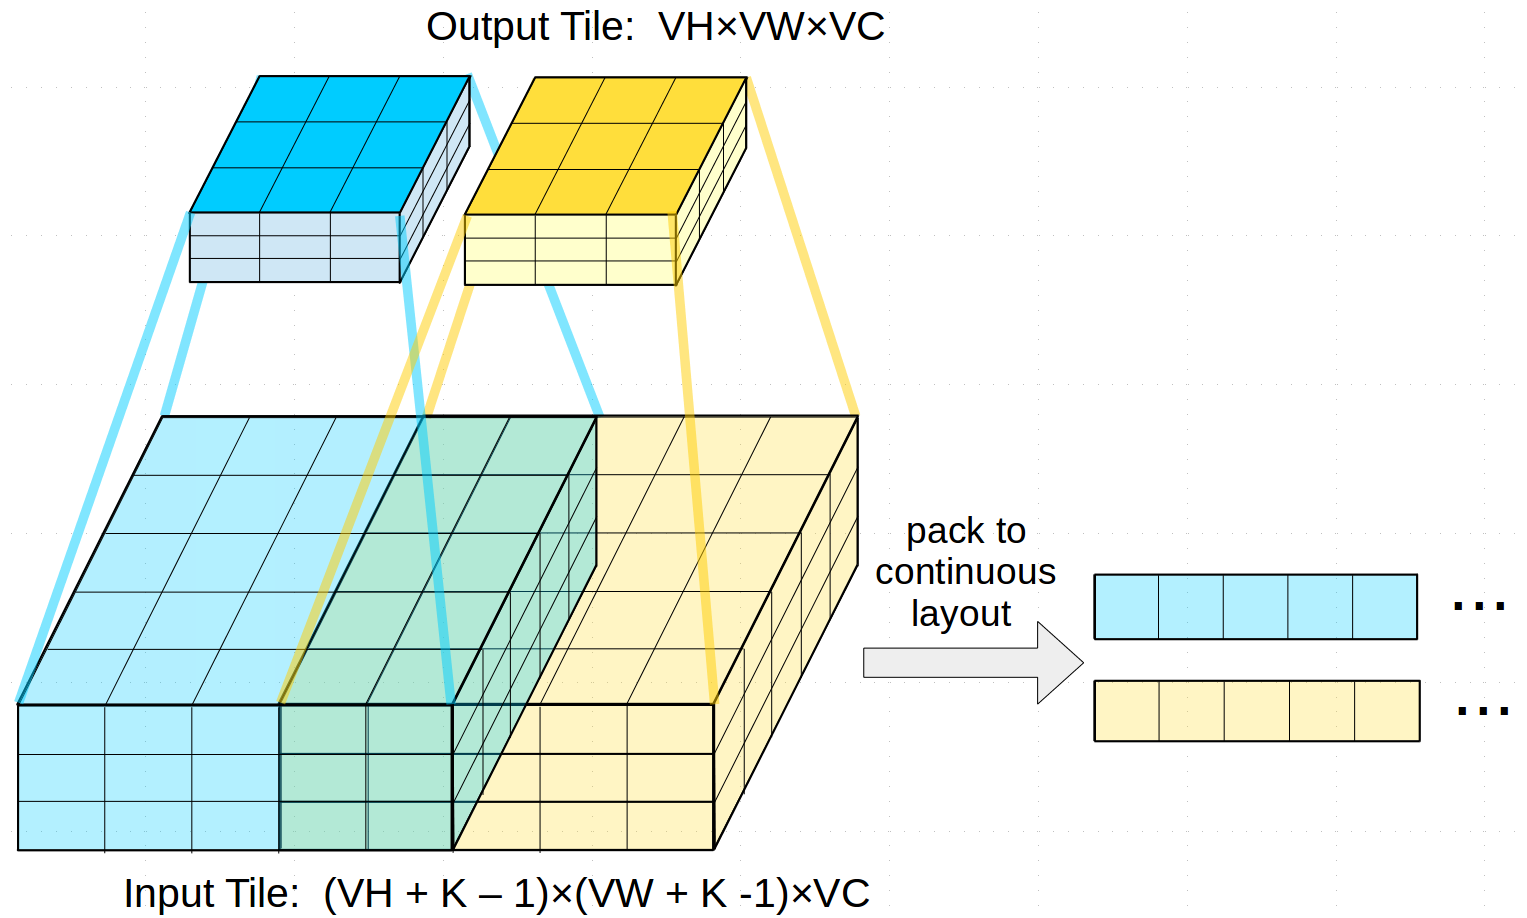
\includegraphics[width=\columnwidth]{figures/spatial.png}
\caption{The Input/Output Tile of Spatial Packing}
\label{fig:tile}
\end{figure}


\begin{figure*}[h]
\centering
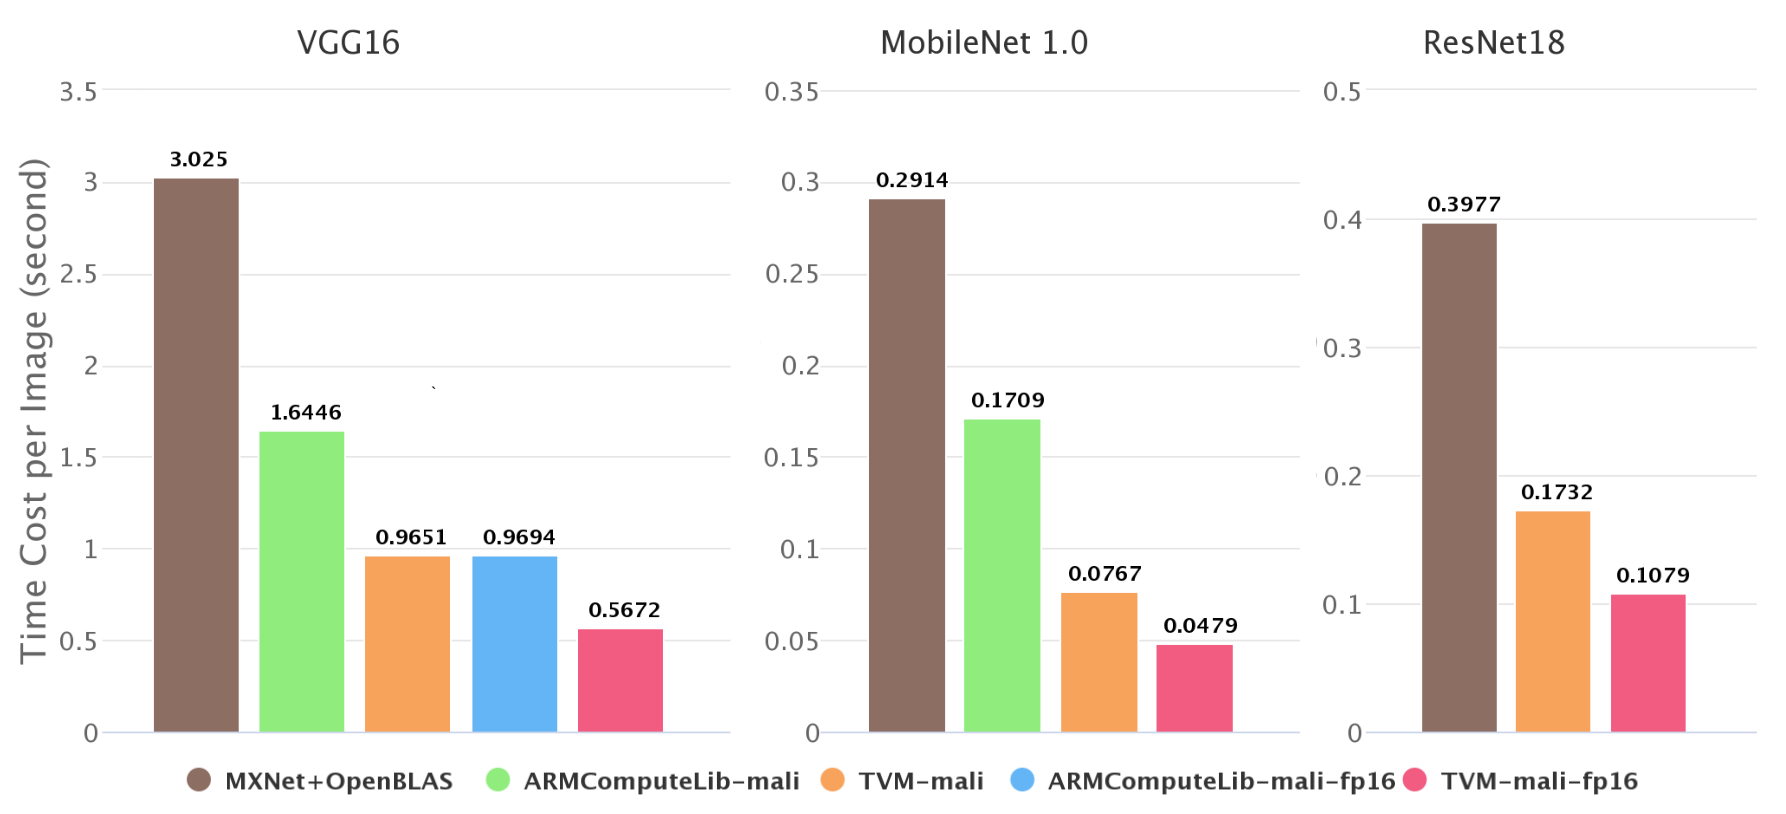
\includegraphics[width=0.9\textwidth]{figures/new_results.png}
\caption{Inference Speed of Different Backends on ImageNet}
\label{fig:end}
\end{figure*}

The memory reduance of this method can be computed by
$$\textbf{memory redundancy} = \frac{(VH + K -1) \times (VW + K - 1)}{VH \times VW}$$
Any configuration  with $VH > 1$ or $VW > 1$ has smaller memory redundancy than im2col. 


\subsubsection{Winograd Fast Convolution for 3x3 Kernel}
Winograd's minimal filtering algorithm has been proven very suitable for convolution layers with small kernel\cite{winograd1980arith, lavin2016fast}. This algorithm can archive the minimal number of float point multiplication for convolution.
For $r\times r$ input data tile  $d$, and $m \times m$ kernel $g$, the convolution is computed by

$$ Y = A^T[[GgG^T] \odot [B^TdB]]A $$

Where $G$ is the transform matrix for data, $B$ is the transform matrix for kernel and $A$ is the inverse transform matrix. We implemented $F(2\times2, 3\times3)$ for convolution layers with 3x3 kernels. See \cite{lavin2016fast} for
 more details of  this algorithm.

\subsubsection{Other Implementation Details}
Because Mali Midgrad GPUs are based on SIMD architecture and need explicit vectorization \cite{armoopenclguide}.
We further try to vectorize and unroll some inner loops, which brings significant speedup.
The shape of workgroup also matters a lot. It controls the memory reuse among threads.
Since there are too many trade-offs in choosing the tile factor and workgroup shape,
we use a tuner to search the optimal values for every layer.

\subsection {Optimizing Depthwise Convolution Layer}
Depthwise convolution layer is a variant of convolution layer. It can greatly reduce the computation complexity of convolution layer, which makes it very suitable for mobile applications \cite{andrew2017mobilenet}. We adopt the similar tiling strategies and get reasonable speedup.

\subsection{Optimizing Dataflow Graph}
This optimization is done by NNVM. The optimization passes include layout transformation, inference simplification,
pre-compute and operator fusion.

\section{Empirical Evaluation}
%{\em Obligatory. Provide empirical evaluation results of the technique together with improved metrics, 
%optimization, or exploration which you are providing an artifact for, and discuss the insights 
%that the evaluation provides. The methodology can be discussed in more details in the artifact appendix.}

Inference speed is the focus in this paper. So we choose time cost per image (batch size = 1) as the metric to evaluate in this section.
We test both single layer performance under various optimization techniques, and end-to-end performance on VGG16, mobilenet and ResNet-18.

\subsection{Test Platform}
We use a commercial ARM board with Rockchip-RK3399 SoC as test environment. 
The detailed information of our test environment is listed below.
\begin{itemize}
\item Board: Firefly-RK3399 4G
\item CPU: dual-core Cortex-A72 + quad-core Cortex-A53
\item GPU: Mali-T860MP4@800Mhz

\item Arm Compute Library : v17.12
\item MXNet: v1.0.1
\item Openblas: v0.2.18
\end{itemize}
To make the environment more stable, we close the GUI on board, and set the `performance' power governor for GPU.

\subsection {Single Layer Comparison}
We take a layer in VGG16 as test case, and investigate the speed up bought by different optimization techniques.
The input shape of this layer is $(C, H, W) = (56, 56, 256)$, and filter shape is $(OC, IC, K, K )= (256, 256, 3, 3)$. As shown in Table. \ref{table:conv2d}, Winograd algorithm is the most efficient one.
\begin{table*}[htbp]
\centering
\begin{tabular}{lccc}
\hline
Kernel & Cost (second) & GFLOPS & speedup \\
\hline
Im2col in ARM CL	& 0.1821 & 20.3111 & 1.00x \\
Spatial Pack: simple bind		& 5.6154	& 0.6588	& 0.03x \\
Spatial Pack: + unrolling		& 0.3707	& 9.9796	& 0.49x \\ 
Spatial Pack: + vectorization		& 0.1304	& 28.3679 & 1.40x \\
Winograd: 		& 0.0819 & 45.1546 & 2.22x \\
\hline
\end{tabular}
\caption{Performance of a convolution layer in VGG16 (ARM CL stands for ARM ComputeLibrary, GFLOPS for Winograd is the effective GFLOPS)}
\label{table:conv2d}
\end{table*}

For depthwise convolution, we measure the time cost of our kernel and ARM CL's kernel for all depthwise  conv layers in mobilenet. 
As listed in Table \ref{table:depth}, ours is faster for all layers.

\begin{table}[h]
\centering
\begin{tabular}{lccc}
\hline
(H, W, C, K) & ARM CL (ms) & Ours(ms) & speedup \\
\hline
(112, 112, 32,   3) & 11.690 & 1.978 & 5.91 \\
(112, 112, 64,   3) & 6.666  & 2.412 & 2.76 \\
(56,  56,  128,  3) & 11.714 & 2.291 & 5.11 \\
(56,  56,  128,  3) & 3.343  & 1.460 & 2.29 \\
(28,  28,  256,  3) & 5.875  & 1.250 & 4.70 \\
(28,  28,  256,  3) & 1.768  & 1.105 & 1.60 \\
(14,  14,  512,  3) & 3.199  & 1.164 & 2.75 \\
(14,  14,  512,  3) & 2.223  & 0.731 & 3.04 \\
(7,   7,   1024, 3) & 3.736  & 0.863 & 4.33 \\
\hline
\end{tabular}
\caption{Performance of Depthwise Convolution Layers}
\label{table:depth}
\end{table}


\subsection {End-to-End Benchmarking}
As shown in Figure \ref{fig:end}, we benchmark the end-to-end performance of different backends. 
Both float32 and float16 precision are measured. Some cases are missing in the plot, because the graph runtime in
 ARM Compute Library currently does not support skip connection.
We try both GEMM and direct method of convolution layer in Arm Compute Library, and GEMM method is always faster than direct method in these test cases, so we only plot the result of GEMM method. 
The results indicate utilizing GPU in this commercial board can be  than 2x \~{}  4x faster than 6-core big.Little CPU. Our end-to-end pipeline
is 1.7x \~{} 2.2x faster then ARM Compute Library.

\section{Conclusion}
In this paper, we implemented  several optimization techniques with TVM/NNVM stack to optimize the inference speed on ImageNet for ARM Mali GPU.
Empirical evaluation results show that our method is faster than vendor-provided ARM Compute Library.


\bibliographystyle{ACM-Reference-Format}
\bibliography{paper}

\newpage

\onecolumn

\appendix
\section{Artifact Appendix}

Submission and reviewing methodology: \\
{\em http://cTuning.org/ae/submission-20171101.html}

%%%%%%%%%%%%%%%%%%%%%%%%%%%%%%%%%%%%%%%%%%%%%%%%%%%%%%%%%%%%%%%%%%%%%
\subsection{Abstract}

This Artifact Appendix describes experimental workflow,
artifacts and results from this paper evaluated 
during the 1st reproducible ReQuEST tournament at the ACM ASPLOS'18:

\begin{packed_itemize}
  \item {\bf Original artifact:} \url{https://github.com/merrymercy/tvm-mali}
  \item {\bf Latest CK workflow:} \url{https://github.com/ctuning/ck-request-asplos18-mobilenets-tvm-arm}
  \item {\bf CK results:} \url{https://github.com/ctuning/ck-request-asplos18-results-mobilenets-tvm-arm}
  \item {\bf Artifact DOI:} \url{https://doi.org/10.1145/3229770}
  \item {\bf ReQuEST submission and reviewing guidelines:} \url{http://cknowledge.org/request-cfp-asplos2018.html} (\cite{request-asplos18})
  \item {\bf ReQuEST goals:} \cite{cm:29db2248aba45e59:0c7348dfbadd5b95}
  \item {\bf ReQuEST workflows:} \url{https://github.com/ctuning/ck-request-asplos18-results}
  \item {\bf ReQuEST scoreboard:} \url{http://cKnowledge.org/request-results}
\end{packed_itemize}

This artifact provides the scripts for the end-to-end benchmarking in the paper.
It benchmarks the inference speed of TVM/NNVM, Arm Compute Library and MXNet + OpenBLAS on
several popular deep neural networks. The image for test is 224x224x3 ImageNet format.

To validate the result,  you can follow our instructions to build these platforms and run test scripts.

%%%%%%%%%%%%%%%%%%%%%%%%%%%%%%%%%%%%%%%%%%%%%%%%%%%%%%%%%%%%%%%%%%%%%
\subsection{Artifact check-list}

Details: \url{http://cTuning.org/ae/submission_extra.html}

{\small
\begin{itemize}
  \item {\bf Algorithm:} image classification
  \item {\bf Program:} TVM/NNVM, ARM Compute Library, MXNet, OpenBLAS
  \item {\bf Compilation:} g++
  \item {\bf Binary:} will be compiled on a target platform
  \item {\bf Data set:} ImageNet 2012 validation (50,000 images)
  \item {\bf Run-time environment:} Linux with OpenCL
  \item {\bf Hardware:} Firefly-RK3399 with ARM Mali-T860MP4 or other boards with ARM Mali GPUs
  \item {\bf Run-time state:} set by our scripts
  \item {\bf Metrics:} inference speed; accuracy
  \item {\bf Output:} classification result; execution time; accuracy
  \item {\bf Experiments:} benchmarking the inference speed of different backends on ImageNet (automated via CK command line)
  \item {\bf How much disk space required (approximately)?:} ~4GB
  \item {\bf How much time is needed to prepare workflow (approximately)?:} several hours (mainly native compilation of packages)
  \item {\bf How much time is needed to complete experiments (approximately)?:} hours for full ImageNet accuracy validation (50000 images)
  \item {\bf Publicly available?:} Yes
  \item {\bf Code license?:} MIT license
  \item {\bf Collective Knowledge workflow framework used?:} Yes
  \item {\bf CK workflow URL:} \url{https://github.com/ctuning/ck-request-asplos18-mobilenets-tvm-arm }
  \item {\bf CK results URL:} \url{https://github.com/ctuning/ck-request-asplos18-results-mobilenets-tvm-arm}
  \item {\bf Original artifact URL:} \url{https://github.com/merrymercy/tvm-mali}
\end{itemize}

%%%%%%%%%%%%%%%%%%%%%%%%%%%%%%%%%%%%%%%%%%%%%%%%%%%%%%%%%%%%%%%%%%%%%
\subsection{Description}

\subsubsection{How to obtain}
The artifact is publicly available on GitHub:  \\
{https://github.com/merrymercy/tvm-mali}

\subsubsection{Hardware dependencies}
Our test hardware is Firefly-RK3399.
Other similar hardwares with ARM Mali T8xx GPU should give comparable results.

\subsubsection{Software dependencies}
Tested platforms TVM/NNVM, Arm Compute Library and MXNet + OpenBLAS  should be built on device. OpenCL Driver is also required.

%%%%%%%%%%%%%%%%%%%%%%%%%%%%%%%%%%%%%%%%%%%%%%%%%%%%%%%%%%%%%%%%%%%%%
\subsection{Installation}
Clone our repository and run the install script.}
\shellcmd{git clone https://github.com/merrymercy/tvm-mali.git}
\shellcmd{cd tvm-mali}
\shellcmd{bash install.sh}

%%%%%%%%%%%%%%%%%%%%%%%%%%%%%%%%%%%%%%%%%%%%%%%%%%%%%%%%%%%%%%%%%%%%%
\subsection{Experiment workflow}
Run the test script and observe the output log in screen. (It needs root permission to set the power governor for GPU)
\shellcmd{sudo bash run\_test.sh}


%%%%%%%%%%%%%%%%%%%%%%%%%%%%%%%%%%%%%%%%%%%%%%%%%%%%%%%%%%%%%%%%%%%%%
\subsection{Evaluation and expected result}

Our evaluation metric is the inference speed on ImageNet 224x224x3 images. The main result 
of this artifact is to reproduce the performance comparison in Figure \ref{fig:end}.
If the reviewer uses the same hardware, we expect the inference time costs in the output log file match the results in our plot.
If other similar hardware is used, we expect the reviewer can observe a similar trend.



%%%%%%%%%%%%%%%%%%%%%%%%%%%%%%%%%%%%%%%%%%%%%%%%%%%%%%%%%%%%%%%%%%%%%
\subsection{Unified installation and evaluation for the ReQuEST scoreboard using Collective Knowledge framework}

\subsubsection{Installation}

**NB:** The `\#` sign means `sudo`.

Install global prerequisites (Ubuntu)

\begin{verbatim}
# sudo apt-get install libtinfo-dev 
\end{verbatim}

\begin{verbatim}
# pip install numpy scipy decorator matplotlib
 or
# pip3 install numpy scipy decorator matplotlib
\end{verbatim}

\textbf{Minimal CK installation}

The minimal installation requires:

\begin{packed_itemize}
 \item Python 2.7 or 3.3+ (limitation is mainly due to unitests)
 \item Git command line client.
\end{packed_itemize}

You can install CK in your local user space as follows:

\begin{verbatim}
$ git clone http://github.com/ctuning/ck
$ export PATH=$PWD/ck/bin:$PATH
$ export PYTHONPATH=$PWD/ck:$PYTHONPATH
\end{verbatim}

You can also install CK via PIP with sudo to avoid setting up environment variables yourself:

\begin{verbatim}
$ sudo pip install ck
\end{verbatim}

\textbf{Install this CK repository with all dependencies (other CK repos to reuse artifacts)}

\begin{verbatim}
$ ck pull repo:ck-request-asplos18-mobilenets-tvm-arm
\end{verbatim}

\subsubsection{Install this CK workflow from the ACM Digital Library snapshot}

It is possible to install and test the snapshot of this workflow 
from the ACM Digital Library without interfering with your current CK installation.
Download related file "request-asplos18-artifact-?-ck-workflow.zip"
to a temporary directory, unzip it and then execute the following commands:

\begin{verbatim}
$ . ./prepare_virtual_ck.sh
$ . ./start_virtual_ck.sh
\end{verbatim}

All CK repositories will be installed in your current directory.
You can now proceed with further evaluation as described below.

\textbf{Detect and test OpenCL driver}

\begin{verbatim}
$ ck detect platform.gpgpu --opencl 
\end{verbatim}


\textbf{Install libBLAS}

\begin{verbatim}
$ sudo apt-get install libblas*
\end{verbatim}

\textit{To detect and register in CK:}

\begin{verbatim}
ck detect soft:lib.blas
\end{verbatim}

\textit{To check the environment:}

\begin{verbatim}
$ ck show env --tags=blas,no-openblas
\end{verbatim}

A possible output:

\begin{verbatim}
cfe1e23a4472bb1d  linux-32  32 BLAS library api-3  32bits,blas,blas,cblas,host-os-linux-32,lib,
                                                     no-openblas,target-os-linux-32,v0,v0.3
\end{verbatim}

\textbf{Install OpenBLAS}

\begin{verbatim}
$ ck install package:lib-openblas-0.2.18-universal
\end{verbatim}

If you want to test other openblas version:

\begin{verbatim}
$ ck list package:lib-openblas* 
\end{verbatim}

\textbf{Install LaPack}

\begin{verbatim}
$ ck install package:lib-lapack-3.4.2
\end{verbatim}

\textbf{Install or detect llvm/clang compiler v4+}

\begin{verbatim}
$ ck install package --tags=compiler,llvm
\end{verbatim}

Though above is the suggested method, you can also install **llvm** via apt and the detect it via CK.

\begin{verbatim}
# apt-get install llvm-4.0 clang-4.0
$ ck detect soft:compiler.llvm 
\end{verbatim}

\subsubsection{Packages installation}

\textbf{ARM Compute Library}

\begin{verbatim}
$ ck install package:lib-armcl-opencl-17.12  --env.USE_GRAPH=ON --env.USE_NEON=ON \
    --env.USE_EMBEDDED_KERNELS=ON 
\end{verbatim}

To check/install other versions available via CK 

\begin{verbatim}
$ ck list package:lib-armcl-opencl-* 
$ ck install package --tags=lib,armcl env.USE_GRAPH=ON --env.USE_NEON=ON \
    --env.USE_EMBEDDED_KERNELS=ON 
\end{verbatim}

\textbf{MXNet with OpenBLAS}

\begin{verbatim}
$ ck install package:lib-mxnet-master-cpu --env.USE_F16C=0
\end{verbatim}

\textbf{NNVM / TVM}

\begin{verbatim}
$ ck install package:lib-nnvm-tvm-master-opencl 
\end{verbatim}

\subsubsection{Original benchmarking (no real classification)}

\textbf{ARM Compute Library client (OpenCL)}

This program must be first compiled

\begin{verbatim}
$ ck compile program:request-armcl-inference 
\end{verbatim}

and then executed as follows:

\begin{verbatim}
$ ck run program:request-armcl-inference --cmd_key=all
\end{verbatim}

You can also use "ck benchmark" command to automatically set CPU/GPU frequency to max, 
compile program, run it N times and perform statistical analysis on empirical characteristics:

\begin{verbatim}
$ ck benchmark program:request-armcl-inference --cmd_key=all
\end{verbatim}

We validated results from the [authors](https://github.com/merrymercy/tvm-mali):

\begin{verbatim}
backend: ARMComputeLib-mali	model: vgg16	conv_method: gemm	dtype: float32	cost: 1.6511
backend: ARMComputeLib-mali	model: vgg16	conv_method: gemm	dtype: float16	cost: 0.976307
backend: ARMComputeLib-mali	model: vgg16	conv_method: direct	dtype: float32	cost: 3.99093
backend: ARMComputeLib-mali	model: vgg16	conv_method: direct	dtype: float16	cost: 1.61435
backend: ARMComputeLib-mali	model: mobilenet	conv_method: gemm	dtype: float32	cost: 0.172009
backend: ARMComputeLib-mali	model: mobilenet	conv_method: direct	dtype: float32	cost: 0.174635
\end{verbatim}

\textbf{MXNet with OpenBLAS client (CPU)}

\begin{verbatim} 
$ ck run program:request-mxnet-inference  --cmd_key=all
 or
$ ck benchmark program:request-mxnet-inference  --cmd_key=all

\end{verbatim}

We validated results from the authors (\url{https://github.com/merrymercy/tvm-mali}):

\begin{verbatim}
backend: MXNet+OpenBLAS	model: resnet18	dtype: float32	cost:0.4145
backend: MXNet+OpenBLAS	model: mobilenet	dtype: float32	cost:0.3408
backend: MXNet+OpenBLAS	model: vgg16	dtype: float32	cost:3.1244
\end{verbatim}

\textbf{NNVM/TVM client (OpenCL)}

\begin{verbatim}
$ ck run program:request-tvm-nnvm-inference  --cmd_key=all 
 or
$ ck benchmark program:request-tvm-nnvm-inference  --cmd_key=all 

\end{verbatim}

We validated results from the [authors](https://github.com/merrymercy/tvm-mali):

\begin{verbatim}
backend: TVM-mali	model: vgg16	dtype: float32	cost:0.9599
backend: TVM-mali	model: vgg16	dtype: float16	cost:0.5688
backend: TVM-mali	model: resnet18	dtype: float32	cost:0.1748
backend: TVM-mali	model: resnet18	dtype: float16	cost:0.1122
backend: TVM-mali	model: mobilenet	dtype: float32	cost:0.0814
backend: TVM-mali	model: mobilenet	dtype: float16	cost:0.0525
\end{verbatim}

\subsubsection{Real classification (time and accuracy)}

Original benchmarking clients did not include real classification in this ReQuEST submission. 
We therefore provided code for real image classification for each of the above CK programs.
This is also required to calculate model accuracy on all (or a subset of) ImageNet data set.

\textbf{MXNet with OpenBLAS client (CPU)}

You can benchmark classification using MXNet with OpenBLAS as follows:

\begin{verbatim} 
$ ck benchmark program:request-mxnet-inference --cmd_key=classify
\end{verbatim}

You can also install ImageNet data sets for model accuracy validation as follows:

\begin{verbatim}
$ ck install package:imagenet-2012-val
or
$ ck install package:imagenet-2012-val-min-resized

$ ck install package:imagenet-2012-aux
\end{verbatim}

You can then run accuracy test as follows:

\begin{verbatim} 
$ ck run program:request-mxnet-inference --cmd_key=test --env.STAT_REPEAT=1
\end{verbatim}

\textbf{NNVM/TVM client (OpenCL)}

You can benchmark classification and test accuracy using TVM/NNVM as follows:

\begin{verbatim}
$ ck benchmark program:request-tvm-nnvm-inference --cmd_key=classify
$ ck run program:request-tvm-nnvm-inference --cmd_key=test --env.STAT_REPEAT=1
\end{verbatim}

\textbf{ARM Compute Library client (OpenCL)}

ReQuEST promotes reusability of AI/ML workflows, packages and artifacts using CK framework. 
Since image classification using ArmCL was already shared as CK workflows and packages 
at \url{https://github.com/dividiti/ck-request-asplos18-mobilenets-armcl-opencl} and added to the ReQuEST scoreboard, 
we can simply reuse this workflow and compare against public results!

Please, follow this ReadME to reproduce ArmCL classification results on Firefly-RK3399: 
\url{https://github.com/dividiti/ck-request-asplos18-mobilenets-armcl-opencl}.

\subsubsection{Validated results}

Validated experimental results were recorded and processed using scripts in the following CK entry:

\begin{verbatim}
$ ck find script:benchmark-request-tvm-arm
\end{verbatim}

We plan to automate them further for the future ReQuEST editions.

\end{document}
